%Copyright 2014 Jean-Philippe Eisenbarth
%This program is free software: you can
%redistribute it and/or modify it under the terms of the GNU General Public
%License as published by the Free Software Foundation, either version 3 of the
%License, or (at your option) any later version.
%This program is distributed in the hope that it will be useful,but WITHOUT ANY
%WARRANTY; without even the implied warranty of MERCHANTABILITY or FITNESS FOR A
%PARTICULAR PURPOSE. See the GNU General Public License for more details.
%You should have received a copy of the GNU General Public License along with
%this program.  If not, see <http://www.gnu.org/licenses/>.

%Based on the code of Yiannis Lazarides
%http://tex.stackexchange.com/questions/42602/software-requirements-specification-with-latex
%http://tex.stackexchange.com/users/963/yiannis-lazarides
%Also based on the template of Karl E. Wiegers
%http://www.se.rit.edu/~emad/teaching/slides/srs_template_sep14.pdf
%http://karlwiegers.com
\documentclass{scrreprt}
\usepackage{listings}
\usepackage{underscore}
\usepackage{graphicx}
\usepackage{svg}
\usepackage[bookmarks=true]{hyperref}
\usepackage[utf8]{inputenc}
\usepackage[english]{babel}
\usepackage{hyperref}
\hypersetup{
    bookmarks=false,    % show bookmarks bar?
    pdftitle={Specification des besoins de programme},    % title
    pdfauthor={VER VALEM Willian BAYOL Elmer LOPEZ-FARFAN M. Liliana TAGNAOUTI Khaoula},                     % author
    pdfsubject={TeX and LaTeX},                        % subject of the document
    pdfkeywords={TeX, LaTeX, graphics, images}, % list of keywords
    colorlinks=true,       % false: boxed links; true: colored links
    linkcolor=blue,       % color of internal links
    citecolor=black,       % color of links to bibliography
    filecolor=black,        % color of file links
    urlcolor=purple,        % color of external links
    linktoc=page            % only page is linked
}%
\def\myversion{1.0 }
\date{}
%\title
\usepackage{hyperref}
\begin{document}

\begin{flushright}
    \rule{16cm}{5pt}\vskip1cm
    \begin{bfseries}
        \Huge{SPECIFICATION DES BESOINS\\ DE PROGRAMME }\\
        \vspace{1.9cm}
        pour\\
        \vspace{1.9cm}
        Dominion Logs Datamining\\
        \vspace{1.9cm}
        Réalisé par \\ VER VALEM Willian \\ BAYOL Elmer \\ LOPEZ-FARFAN M. Liliana
        \\ TAGNAOUTI Khaoula\\
        \vspace{1.9cm}
        \today\\
    \end{bfseries}
\end{flushright}

\tableofcontents


% \chapter*{Revision History}

% \begin{center}
%     \begin{tabular}{|c|c|c|c|}
%         \hline
%       Name & Date & Reason For Changes & Version\\
%         \hline
%       21 & 22 & 23 & 24\\
%         \hline
%       31 & 32 & 33 & 34\\
%         \hline
%     \end{tabular}
% \end{center}

\chapter{Contexte}

\section{Introduction}
Le jeu de cartes \textit{Dominion} a été mis à disposition sur un serveur de jeu d'octobre 2010 à mars 2013. Les parties effectuées via ce serveur ont été enregistrées dans des \textit{logs} qui mémorisaient toutes les actions des joueurs ; ces \textit{logs} ont été mis à disposition du public. Mais ces enregistrements n'ont pas conservé un certain nombre d'informations ayant un rapport avec les décisions prises par les joueurs.
\newline Un wiki relatif au jeu a été élaboré, et propose des avis d'experts comme aide à la décision pour les joueurs : il propose des conseils, notamment au niveau stratégique. Le but de ce projet, proposé par Yvan Le Borgne, chercheur au Labri, est de traiter ces \textit{logs} (soit plus de 12 millions de parties) afin de répondre à plusieurs interrogations. Il s'agira principalement de comparer Les données recueillies aux préconisations de ce wiki,afin de valider, à travers les contenus des parties, l'éventuelle efficacité des avis et suggestions fournies par les experts. A tout le moins, on cherchera à élaborer des outils de validation présentant une efficacité suffisante.
\newline Dans cette optique, le projet a pour but de créer une base de données recensant les parties puis un travail d'analyse sera effectuée à partir de celle-ci.
Pour cela notre programme devra tout d'abord extraire les données présentes dans les logs, car ceux-ci sont trop volumineux et trop compliqués à utiliser directement (structure non standardisée). Il s'agira de mettre au point des structures de données permettant de stocker les données de manière plus efficace. Une manière simple de représenter les données extraites et analysées sera proposée à l'utilisateur.
Par ailleurs, il manque des informations dans les enregistrements (\textit{logs}). On cherchera à trouver par quelle méthode on peut les reconstituer et de les mettre dans un format contenant toutes les informations.
En outre, on cherchera à optimiser les opérations menées dans l'analyse des donnnées, en recherchant le meilleur équilibre possible entre la mémorisation des recherches et le re-calcul.
Enfin, on esssaiera de déterminer quelle stratégie a été utilisée dans chaque partie. Voire de faire émerger les changements de stratégie en cours de partie. Si on prend pour exemple une des stratégies (la \textit{Penultimate Province Rule}) peut on détecter à quel moment cette règle a été appliquée ou contournée ? ou qui a mis au point cette stratégie ? (découverte qui pourrait permettre d'organiser un classement des joueurs les plus performants) (une sorte de ELO demandé par le client). Dans la mesure où on parviendrait à mettre au point un nombre suffisant de ces démarches stratégiques, il s'agirait de déterminer le processus habituel d'apprentissage des joueurs.

\section{Règles du jeu}
Chaque joueur possède un deck de cartes et a accès à un <<marché>> ou différentes cartes d'action sont disponible. Il y a également une pile de cartes de victoires.
\newline Les joueurs commencent avec un deck contenant uniquement des cartes de monnaie permettant d'acheter les autres cartes mises à la disposition des joueurs. Les joueurs commencent leur tour avec 5 cartes en main et le tour d'un joueur se déroule en deux phases, premièrement la phase d'action, le joueur peut jouer une carte d'action, puis une phase d'achat ou le joueur peut acheter des cartes du marché, des cartes de monnaie ou des cartes de victoires.
\newline La partie se termine dans deux cas, si la réserve de cartes <<Province>> (carte de victoire au score le plus élevé) est vide ou bien si 3 piles du marché sont vides. Quand la partie est terminée, les points de victoires (découlant des cartes de victoire) de chaque deck sont comptés et le vainqueur est celui qui à la meilleur score.

\section{Analyse de l'existant}
goko-dominion-tools est le principal outil disponible pour exploiter les logs, mais cette version ne fonctionne plus car les serveurs goko ont été fermés. Les fonctionnalités offertes par cet outil sont très proches de ce que nous voulons proposer, notamment un parsing de logs, une recherche dans ces logs et un leaderboard. Le programme est écrit en python et est disponible sur github.
%TODO: chercher quelques bots à présneter

\chapter{Analyse du besoin}

\section{Objectif}

Ce document a pour but de clarifier et de décrire aussi précisément que possible les besoins pour le développement du programme \textit{Dominion DataMining}.\\
\textit{Dominion DataMining} est un programme qui se compose de 3 parties:

\begin{itemize}
  \item \textbf{Modélisation des donnée:} \- responsable de la lecture et du remodelage des données à stocker.
  \item \textbf{Stockage de données:} \- stocke les données analysées.
  \item \textbf{Analyse des données:} \- effectue les requètes vers la base de données et traite les données stockées.

\end{itemize}


 \section{Public visé et suggestions de lecture}

Ce document est destiné à tout utilisateur, développeur, testeur, chef de projet ou écrivain de documentation qui a besoin de comprendre l'architecture de base du système et de ses spécifications.\\
Voici les utilisations potentielles pour chacun des types de lecteurs:\\
\begin{itemize}

\item \textbf{Développeur: }le développeur qui veut lire, changer, modifier ou ajouter de nouveaux besoins dans le programme existant, doit tout d'abord consulter ce document et mettre à jour les besoins en manière appropriée afin de ne pas détruire leur signification réelle et de transmettre des informations correctement aux prochaines phases du processus de développement.\\

\item \textbf{Utilisateur: }l'utilisateur de ce programme fait la revue des schémas et les spécifications présentées dans ce document et détermine si le logiciel a tous les besoins appropriés et si le développeur du logiciel a mis en œuvre tous.\\

\item \textbf{Testeur: }le testeur a besoin de ce document pour vérifier que les besoins initiaux de ce programme correspondent actuellement  au programme exécutable correctement.\\
\end{itemize}

\section{Contexte du projet}
  Le jeu de cartes\textit{Dominion} a été hébergé sur un serveur à partir d'Octobre 2010 à Mars 2013. Les parties jouées sur ce serveur ont été enregistrés dans des \textit{logs} qui gardent la trace de toutes les actions des joueurs;ces \textit{logs} ont été mis à la disposition du public. Mais certaines informations par rapport aux décisions prises par les joueurs n’ont pas été enregistrées.\\
 Un wiki sur le jeu a été créé, il offre des conseils d'experts dans la prise de décision au cours du jeu: il offre principalement des conseils au niveau de la stratégie. Le but de ce projet, proposé par Yvan Le Borgne, chercheur au Labri, est de traiter des \textit{logs} (plus de 12 millions de parties) afin de répondre à plusieurs questions. Il consiste principalement à comparer les données recueillies à l'information du wiki afin de valider l'utilité des idées et des informations données par des experts. Nous allons au moins créer des outils de validation offrant suffisamment efficaces.
  
Afin d'Atteindre cet objectif, le but du projet est de créer une base de données contenant tous les jeux joués et de produire une analyse basée sur ces informations. Pour ce faire, notre programme devra d'abord extraire les données des \textit{log}, car ils sont trop volumineux et trop compliqués à utiliser directement (structure non-standard). Nous aurons à mettre en place des structures de données qui nous permettent d'avoir un meilleur stockage de données. Un moyen simple pour représenter ces données sera offert à l'utilisateur.

  Certaines informations sont également manquantes dans les \textit{logs}(par exemple: les cartes piochées au cours d'un tour). Nous allons essayer de trouver une méthode pour reconstruire cette information et l'ajouter à l'information existante. Nous allons également essayer d'optimiser les opérations effectuées par l'analyse de données en trouvant un équilibre entre la mémorisation des demandes et le recalcul.

  Enfin, nous devrons décider quelle stratégie est utilisée avec chaque jeu, ou même reconnaître les changements de stratégie lors d'un match. Nous pourrions aussi reconnaître qui a appliqué une première stratégie (qui l'a \textit{inventé}). Si nous pouvons détecter assez  stratégie liée aux données, nous pouvons également détecter le processus d'apprentissage d'habitude des joueurs.


\section{Description globale}


\section{Fonctions de produit}

Voici une liste des fonctions qui devraient être disponibles sur le logiciel:
\begin{itemize}

%\item{\textbf{Interface utilisateur:}}

 %   \begin{itemize}
  %  \item{Lancement de log analysé}
   % \item{Statistiques demandés}
    %\item{Mappage des données de jeu}
    %\end{itemize}
  \item{\textbf{Modélisation des données:}}
    \begin{itemize}
    \item{Décompression de log}
    \item{Parsing}
    \item{Creation de game-log}
    \item{Envoi de game-log data}
    \end{itemize}
  \item{\textbf{Stockage de données:}}
    \begin{itemize}
    \item{Créer une base de données orientée document}
    \item{Se connecter à la base de données orientée document}
    \item{Compression}
   % \item{charger le game-log}
    \item{Enregistrer le game-log}
    \end{itemize}
  \item{\textbf{Analyse des données:}}
    \begin{itemize}
      \item{Recueillir les données}
      \item{Restorer le game-log}
      \item{Plotting}
      \item{Calculer \textit{\textbf{ELO}}}
      \item{Reconnaître les stratégies}
      \item{Reconnaître Greening}
    \end{itemize}
\end{itemize}
\textit{ Une description plus précise de chaque fonctionnalité sera disponible dans la section 4 de ce document. }
\section{Classes de l'utilisateur et caractéristiques}

\textbf{Acteurs physiques:}\\

\begin{itemize}
 \item \textbf{Utilisateur:} l'utilisateur lance l'analyse des logs et des demandes des analyses à faire sur les données stockées qui seront ensuite représentées sous forme de graphes.\\
   Les actions de l'utilisateur peuvent être décomposées en deux parties:
   \begin{itemize}
   \item Étape de pré-calcul: %Cette action sera réalisée une fois au début et lancera la phase de l'analyse et de l'analyse classique des jeux(Reconnaissance de la stratégie, le calcul elo).
   \item Les données de l'analyse de l'utilisateur: une librairie en python sera offerte à l'utilisateur, pour qu'il puisse demander l'affichage des statistiques standard ou créer analyse complexe en utilisant son propre programme python assoscié à une bibliothèque proposant diverses fonctions. 
   \end{itemize}
\end{itemize}

\textbf{Acteurs de Système:}\\
\begin{itemize}
 \item \textbf{Parser :} le parser est le système qui a accès en écriture à la base de données et est responsable du stockage des données analysées sur la base de données.

 \item \textbf{Analyzer :} l'analyseur est le système qui va interroger la base de données pour recueillir des données pour l'analyse, et sera en mesure de créer des requêtes persistantes.

   \item \textbf{Base de données: } La base de données stocke les données extraites des logs et réponds aux requêtes des autres parties du programme.
\end{itemize}

\textit{Le logiciel à développer est destiné à un usage personnel, il n'y a donc pas d'accès privilégié, l'utilisateur aura accès à l'intégralité du code et des données.}
\section{Conception et mise en œuvre Contraintes}
Cette section présente un aperçu des problèmes possibles qui peuvent limiter le développement du logiciel:
\begin{itemize}
\item Le logiciel sera développé pour le système d'exploitation Linux et aucune autre plate-forme n’est nécessaire.
\item Le logiciel doit fonctionner sur le matériel trouvé sur de simples ordinateurs personnels.
\item Les données à analyser sont considérablement grandes (400Gb) et le client ne sera pas en mesure de fournir un serveur afin de travailler avec les données non compressées ce qui peut avoir un impact sur les performances du logiciel.

\item Les \textit{Logs} fournis ne sont pas a un format standard ce qui peut retarder le temps de développement l'analyseur les problèmes qu'il peut soulever au cours du développement ne sont pas connus pour le moment.
\end{itemize}

\section{Les logs}
\subsection{Description des données}
Les données qui ont été fournies par le client sont compressées en format tar.bz2, un fichier pour chaque jour de log, la taille totale des données compressée est 13 Go.\\
Les données décompressées font un total de 400 Go.\\
Chaque \textit{Log} est au format \textit{HTML}.\\
un \textit{Log} doit contenir:
\begin{itemize}
  \item{\textbf{en-tête:}} contient le numéro de jeu et les noms des gagnants.
  \item{\textbf{résumé de  match:}} contient les cartes utilisées sur le match et comment le match a fini.
  \item{\textbf{résumé de joueur:}} contient  les cartes de victoire de chaque joueur,le deck et les points.
  \item{\textbf{game log:}} cette partie contient tous les actions détaillées effectuées par les joueurs pendant le match.

\end{itemize}

\subsubsection{Incohérence des données}
Les \textit{Logs} présentent des incohérences de données qui peuvent être problématiques lors du développement de l'analyseur. Voici quelques exemples de problèmes rencontrés:

\begin{itemize}
  \item \textbf{Numéro de log}\\
   La numérotation des logs n'est pas unique ce qui implique qu'elle ne peut pas être utilisée pour identifier un log.
  \item \textbf{Noms d'utilisateur}\\
    Les logs montrent qu'aucune restriction n’a été fait sur les noms d'utilisateur du jeu et quelques noms d'utilisateur ont des mots clés et des caractères spéciaux qui peuvent entrer en conflit avec l'analyseur.
   \item \textbf{Données manquantes}\\
    Certains des logs ont une partie des données manquantes (comme: l'en-tête, la reprise des utilisateurs $\ldots$).
   \item \textbf{Format de log}\\
    La syntaxe utilisée lors de l'écriture des logs peut varier.
    %\item \textbf{Compression de données}\\
     %Comme les données sont compressées et l'équipement fourni à travailler sur le projet ne peut pas gérer les données non compressées, le projet va travailler avec des données compressées, et après un premier indice de référence, 4 heures a été nécessaire pour décompresser.
\end{itemize}

\section{Besoins fonctionnels}
\iffalse
\section{Interface utilisateur}
%TODO: retravailler cette portion
L'interface utilisateur du programme sera composé d'un exécutable (minière de domination) qui sera exécuté avec certains paramètres pour exécuter l'action souhaitée. Le schéma ci-dessous représente les différentes interactions disponibles pour l'utilisateur:\\

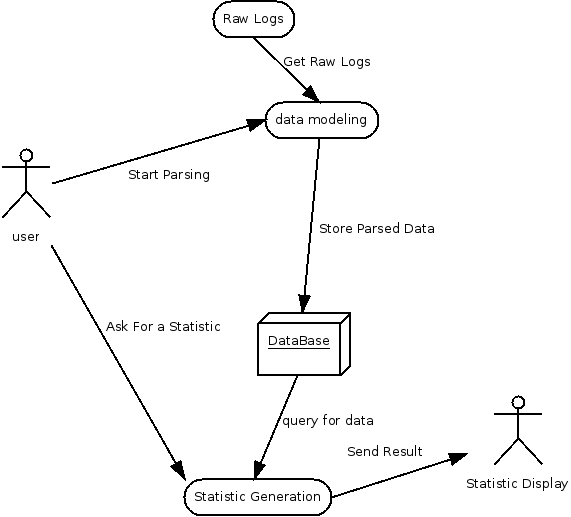
\includegraphics[scale=0.45,keepaspectratio]{diaRessources/UseCaseParsing}\\
Avant l'utilisation de toutes les fonctionnalités du programme, l'utilisateur doit lancer l'analyse.
\subsection{Lancement de l'analyse du log}
\subsubsection{Description et priorité}
\textbf{Niveau de priorité = haute}\\
\begin{itemize}
  \item L'utilisateur devra placer tous les logs compressés (fichiers tar.bz2) pour être analysées dans un dossier spécifique.
  \item si aucune compression est donnée la compression par défaut est \textit{snappy}.
    \item Pour des fins de test, afin d'éviter d'avoir un 4 heures étape d'analyse, l'utilisateur peut spécifier un pourcentage des logs pour être analysée. en spécifiant une valeur comprise entre 0 et 100. l'analyseur choisira au hasard les logs de ceux qui sont prévus et les analyser, en créant une base de données utilisable pour des tests supplémentaires.
    \item Une fois que l'analyse est effectuée un message sera affiché sur la console (traitement de fait).

\end{itemize}

\subsection{Statistiques demandées}
\subsubsection{Description et priorité}
\textbf{Niveau de priorité = haute}\\
La demande d'une statistique peut être faite en tapant les états de \textit{dominionmining (paramètres)}.  \\
Les noms de stratégie possibles sont: big money, pen province, beyond silver.\\
Si d'autres stratégies sont reconnues par le programme, ils seront ajoutés à la liste.\\
La liste des paramètres qui seront possible d'utiliser sera déterminée dans le futur.\\

Le retour d'une statistique peut être un graphique affiché dans une fenêtre ou exportés vers un fichier. Si sa une valeur unique, un nom ou une phrase, il sera retourné à l'invite.

\subsection{Mappage des données de jeu}

Afin de permettre à l'utilisateur de demander des statistiques spécifiques concernant un jeu, le programme peut être exécuté afin de générer des logs de jeu simplifiées et un script python sera appliqué à ce log. Cela permettrait une plus grande flexibilité dans le type de statistiques affichables par le programme.
\begin{itemize}
\item Le programme sera lancé en utilisant la commande suivante: \textit{dominionmining data\_to\_query user\_script.py}
 \item Le script python sera appliquée au résultat généré et retourner les statistiques demandées par l'utilisateur.
\item Le fichier généré contenant les résultats de la requête aura le format suivant:
\begin{itemize}
\item Le nom du fichier produit est \textit{game.txt}
\item Le log simplifié contiendra chaque action effectuée par le joueur, une action par ligne. Liste des actions et leur format:
\begin{itemize}
\item Révéler une carte: \textit{joueur\_x révèle carte\_nom}
\item Piocher des cartes: \textit{joueur\_x jete n cartes}
\item Acheter une carte: \textit{joueur\_x buys carte\_name}
\item Jeter des cartes: \textit{joueur\_x trashes n cartes}
\item Mettre une carte \textit{joueur\_x puts carte\_name}
\item Gagner une carte: \textit{joueur\_x gains carte\_name}
\item Jouer une carte: \textit{joueur\_x jouer une carte\_name}

\end{itemize}
\end{itemize}
\end{itemize}
\fi
\section{Modélisation des données}

\subsection{Décompression des logs}
\subsubsection{Description et priorité}
\textbf{Niveau de priorité = haute}\\
\begin{itemize}
  \item Les fichiers tar.bz2 seront stockés dans un dossier.
  \item Le programme va  décompresser un fichier spécifié à partir de ce dossier dans un dossier temporaire.
  \item Le programme va  supprimer les logs décompressés  à la demande du parser.
\end{itemize}

\subsection{Parser}

\subsubsection{Description et priorité}
\textbf{Niveau de priorité = haute}\\
L'analyseur va prendre les logs sous format \textit{HTML} et va identifier les mots clés présents sur ces logs.\\
L'analyseur est chargé de lire les logs et collecter l'information importante sans perdre la structure du log.\\
Un aperçu des données pour être reconnu par l'analyseur est illustré dans ce diagramme:\\

\includegraphics[scale=0.35,keepaspectratio]{diaRessources/UseCaseParser}

\begin{itemize}
\item Winners: liste des gagnants du jeu, il peut y avoir plusieurs gagnants en cas d'égalité.
\item Market: liste des 10 cartes disponibles pour être acheté par les joueurs.
\item Cards Gone: liste des cartes qui ont été entièrement acquises à la fin de la partie.
\item Player Name: Nom du joueur.
\item Victory points: nombre de points à la fin de la partie.
\item Player cards: liste des cartes obtenues à la fin de jeu avec des noms et de quantités differents.
\item Victory cards: liste des cartes de victoire le joueur avec le acheté.
\item Trash: liste des cartes qui sont jetés à la fin de la partie.
\item Game Moves: liste des actions effectuées pendant chaque tour d'un joueur.
\end{itemize}
Le parser doit lire chaque élément montré dans le graphique précédent en tant que partie des données lorsque l'utilisateur exécute le programme de parsing\\

\subsection{Créer game-log}
\subsubsection{Description et priorité}
\textbf{Niveau de priorité = haute}\\
Cette fonctionnalité est la création d'une structure de données où les données du log seront écrites.
Voici une représentation graphique d'une vue d'ensemble de la structure de données:\\
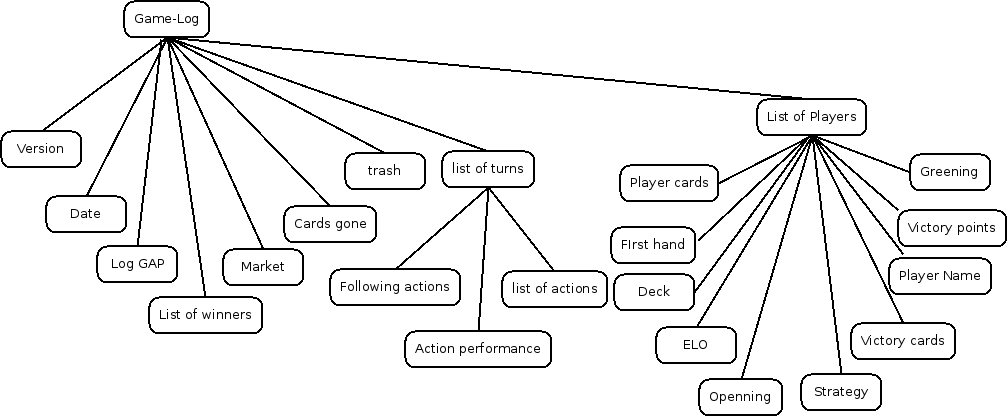
\includegraphics[scale=0.5,keepaspectratio]{diaRessources/game-log}

\subsection{Créer une base de données orientée document }

\subsubsection{Description et priorité}
\textbf{Niveau de priorité = haute}\\
Ce module sera responsable pour créer la base de données orientée document, contenant des données au format JSON.
\subsection{Se connecter à la base de données orientée document }
\subsubsection{Description et priorité}
\textbf{Niveau de priorité = haute}\\
\begin{itemize}
\item La base de données orientée document sera en charge des échanges à travers un socket spécifique.
\item La base de données orientée document recevra les logs de jeu au format JSON.
\item La base de données orientée document recevra les demandes du programme relatif à chaque élément de données qu'il contient.
\item La base de données orientée document enverra les résultats des demandes effectuées par le programme.
\end{itemize}


\subsection{Compression}
\subsubsection{Description et priorité}
\textbf{Niveau de priorité = moyen}\\

La base de données orientée document contiendra la plupart des données et un certain niveau de compression devra être appliquée.
La base de données que nous allons utiliser est focalisé sur mongodb, et il offre 2 niveaux de compression \textit{Zlib} et \textit{Snappy}.
Au cours du développement \textit{Snappy} est utilisé car il offre une meilleure performance.
Mais le programme final devrait donner à l'utilisateur la possibilité de choisir le niveau de compression lors du démarrage de l'analyse du log.

\subsection{Sauvegarder game-log}

\subsubsection{Description et priorité}
\textbf{Niveau de priorité = haute}\\
\begin{itemize}
\item La base de données orientée document permet de convertir la structure log de jeu dans un document au format JSON.
\item Les données fournies au format JSON seront stockées dans la base de données.
\end{itemize}
%partie de python à discuter
\section{Analyse des données}
\subsection{Recueillir des données}
\subsubsection{Description et priorité}
\textbf{Niveau de priorité = haute}\\
\begin{itemize}

\item L'analyseur de données va convertir les résultats de la requête dans un format utilisable par le module de traçage.
\item Si les données sont simples à lire (par exemple: un numéro, un nom, une phrase), l'analyseur de données sera tout simplement envoyer le résultat au format texte.
\item La dernière requête sera mémorisée avec son résultat afin de gagner du temps si la prochaine requête faite par l'utilisateur est le même.
\item Si l'utilisateur souhaite appliquer un script python de logs de jeu, le programme demandera les logs de jeu et les mettre dans un fichier texte, ce fichier contiendra chaque action faite par chaque joueur et le script sera appliqué à ce fichier.
\end{itemize}

\subsection{restorer game-log}
\subsubsection{Description et priorité}
\textbf{Niveau de priorité = moyen}\\

Cette fonction est responsable pour restaurer l'information manquante sur les logs analysés, en utilisant la déduction basique sur la base des données obtenues par le log.\\
En cas d'un en-tête du jeu manquant ou partie manquante:
  \begin{itemize}
\item Gagnants / cartes de victoire / points de victoire manquant: le programme peut garder la trace des cartes détenues par les joueurs pendant le jeu afin de savoir combien de cartes victoire qu'ils ont à la fin de la partie.
\item Market manquant: Le programme peut garder la trace des cartes achetées au cours du jeu afin de reconstituer partiellement ou totalement les cartes disponibles sur Market.
\item Cartes Gone: Comme avec les données manquantes de Market, le programme permet de garder une trace de cartes achetées et compter la quantité achetée pour chaque carte, si le montant maximum de cartes est acheté, la carte a disparu à la fin de la partie.
\item Nom du joueur manquant: le jeu se déplace partie d'un log assure également le suivi des noms des joueurs, le programme sera tout simplement de les restaurer dans l'en-tête.
\item Cartes de joueur: le programme permet de garder une trace des actions effectuées au cours du jeu par rapport aux cartes de joueurs et les ajouter dans cette liste.
  \end{itemize}

\subsection{Plotting}
\subsubsection{Description et priorité}
\textbf{Niveau de priorité = haute}\\

Le module de traçage va obtenir les données converties obtenues après le processus de recueillir des données et de les tracer dans une interface graphique. Ce module va fonctionner d'une manière similaire de \textit{GnuPlot}.

\subsection{Calculater \textit{\textbf{ELO}}}
\subsection{Plotting}
\subsubsection{Description et priorité}
\textbf{Niveau de priorité = haute}\\

L'analyseur devra calculer la finale ELO pour chaque joueur et ce qui était un joueur ELO sur un jeu donné.
Pour chaque jeu dans l'ordre chronologique, ce module va demander au elo initiale des joueurs de la base de données relationnelle et les gagnants du jeu, puis il va calculer la nouvelle elo de chaque joueur de l'issue du jeu. Le module sera ensuite définir le elo calculés dans la base de données orientée documents au jeu en cours d'analyse et mettra également à jour l'elo globale pour chacun des joueurs qui participent au jeu sur la base de données relationnelle.\\

Plus d'informations sur ELO peuvent être consultés sur \url{https://en.wikipedia.org/wiki/Elo_rating_system}\\
Le schéma suivant illustre le processus du calcul de elo:\\
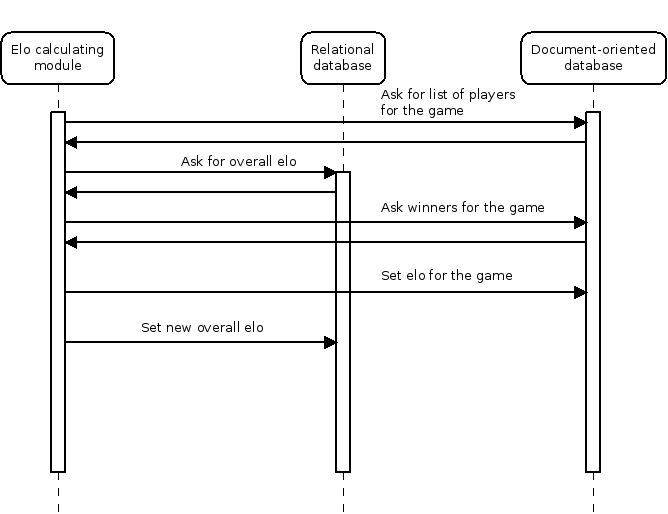
\includegraphics[width=\textwidth,height=\textheight,keepaspectratio]{diaRessources/elocalc}\\

\subsection{Reconnaître les stratégies}
\subsubsection{Description et priorité}
\textbf{Niveau de priorité = moyen}\\

Le wiki de dominion décrit quelques stratégies qui peuvent être utilisés dans le jeu.\\Par exemple :\\
Big Money\\
Beyond Silver\\
Penultimate Province Rule\\
Pour plus de détails sur \url{http://wiki.dominionstrategy.com/index.php/Strategy}\\



\textbf{Cette image décrit le processus de décision associé à la stratégie Big Money}\\
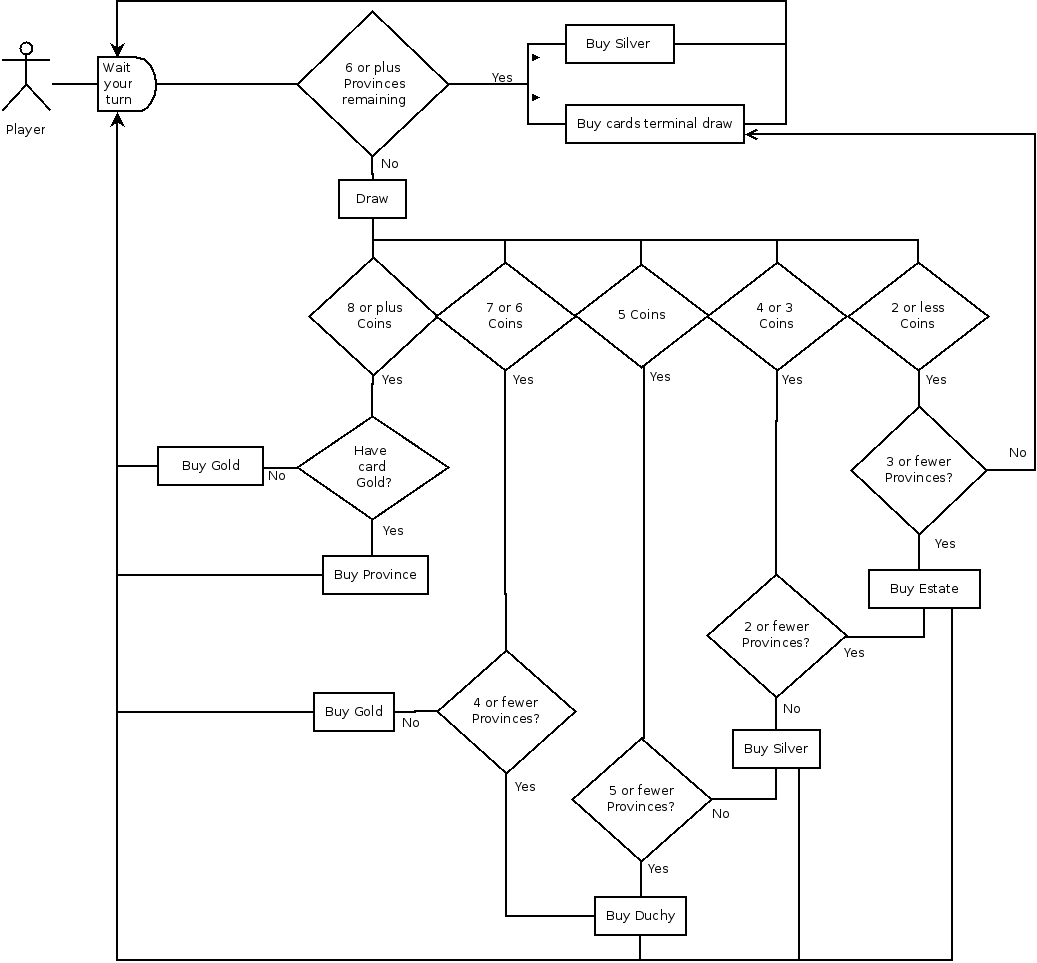
\includegraphics[width=\textwidth,height=\textheight,keepaspectratio]{diaRessources/big-money}\\
%The analyzer has to recognize when a player buys only money cards and specific cards related to the big money strategy. It also has to keep track of the remaining provinces to be bought.\\
Et l'analyseur devra être en mesure de reconnaître quelle stratégie a été utilisée sur un match donné (si une  stratégie a été utilisée) et générer des statistiques.\\
Plus de détails \url{http://wiki.dominionstrategy.com/index.php/Big_Money}\\

Afin de reconnaître la stratégie inventé Beyond Silver, l'analyseur doit reconnaître lorsque certains types de cartes sont achetés, la liste de ces cartes peuvent être trouvés sur : \url{http://wiki.dominionstrategy.com/index.php/Silver#Beyond_Silver}\\

Afin de reconnaître que Penultimate Province Rule est respecté (comme expliqué à \url{http://dominionstrategy.com/2011/03/28/the-penultimate-province-rule/}), l’analyseur doit garder une trace de la quantité de Points de Victoire de chaque joueur à chaque tour.

\subsection{Reconnaître Greening}
\subsubsection{Description et priorité}
\textbf{Niveau de priorité = haute}\\

L'analyseur doit être capable de reconnaître le moment de \textit{\textbf{greening}} sur chaque match.
En savoir plus à propos de \textit{\textbf{greening}} sur \url{http://wiki.dominionstrategy.com/index.php/Greening}.\\
Le programme va reconnaître quand greening arrive en détectant lorsque les cartes de victoire commencent à être achetées.

\section{Besoins non fonctionnelles }
\section{Besoins de performance}

Aucun besoin de performance spécifique n’a été faite par le client. Mais pour l'analyseur le temps d’exécution  doit être inférieur à une heure.\\
L'utilisateur doit être capable de parcourir le processus d'analyse sur un ensemble de données précis sans devoir attendre que la même requête à refaire.

\section{Fiabilité}

Le client demande que le nombre maximum de log doivent être analysé, que les données fournies ont des incohérences et quelques logs ne seront pas possibles d'analyser.\\
L'analyseur devra analyser 100\% des données présentes sur le log et restaure toute information manquante si possible.\\
\section{Attributs de qualité de logiciels}

Même si seulement une ligne de commande est prévue pour le programme final, elle devrait avoir une courbe facile à apprendre et être facile à utiliser.\\
Les données générées par l'analyseur n’ont pas besoin à être lisible par l'homme.\\
Les game log générés devront être analysés par l'utilisateur afin de permettre la plus grande souplesse possible dans le traitement des logs.

\section{Besoins organisationnels}

La répartition des tâches du projet et l'estimation de la durée de chacune d'elle sont présentées sur le planning suivant:\\

\section{Planning prévisionnel}

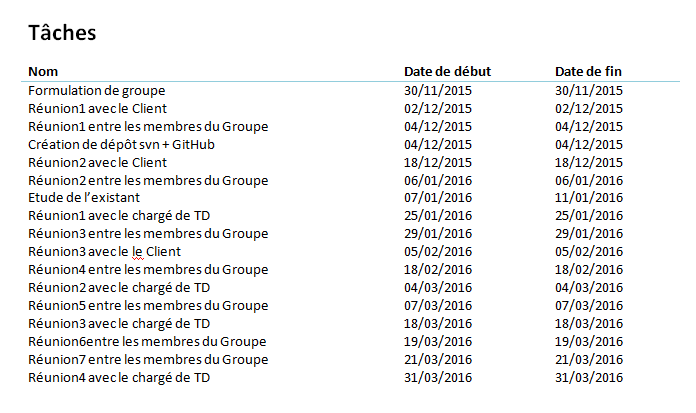
\includegraphics[scale=0.45,keepaspectratio]{planning}\\

\section{Diagramme de Gantt}

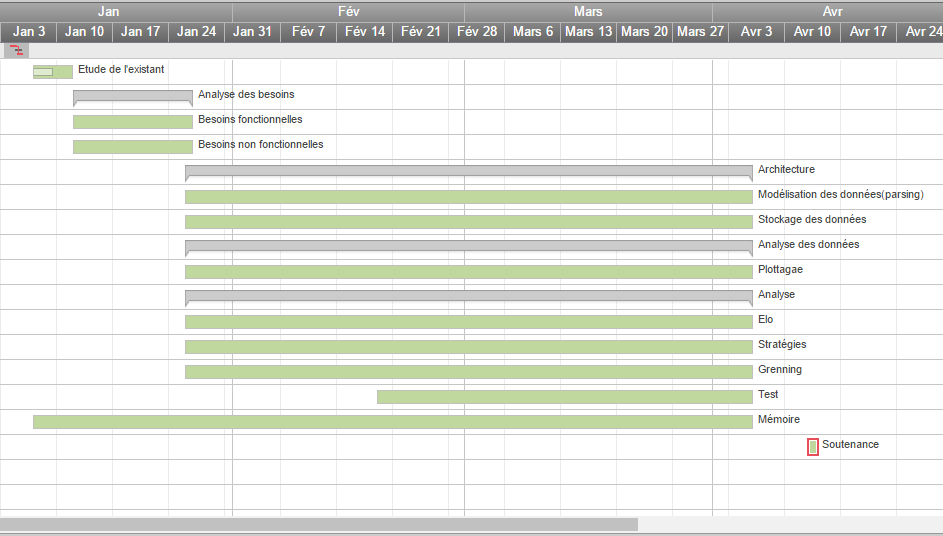
\includegraphics[scale=0.45,keepaspectratio]{gantt}\\

\chapter{Architecture et description du logiciel}

\section{Structure des classes}


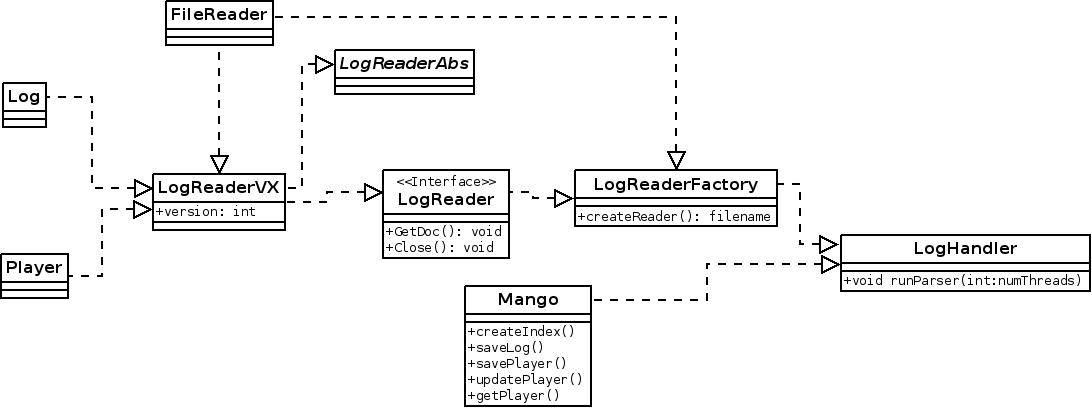
\includegraphics[scale=0.45,keepaspectratio]{diaRessources/nouvelleArch}\\


\chapter{Fonctionnement et tests}
\section{Fonctionnement de programme}
\section{Test}
\chapter{Bibliographie}
\bibliography{biblio}
\end{document}
